%!TEX root = thesis_name.tex

% for wirting a thesis: use book and openright with twoside!
\documentclass[11pt, a4paper, twoside, openright, final]{book}

%%% input encoding
\usepackage{ucs}				% contains support for using UTF-8 as input encoding. Could in most cases be ommited
\usepackage[utf8x]{inputenc}	% use utf8 as document encoding.
								% Therefore, umlaute (ä,ö,ü,ß,...) could be used as they are, without any special latex commands

%%% language
\usepackage[german]{babel}	% english hyphonation and english as default language
								% change here to "ngerman" for automatic translation from "figure" to "Abbildung" and so on
\usepackage[german=guillemets]{csquotes} % German guillemets quotes

%%% better readable fonts
\usepackage{libertine}					% standard font
\usepackage[scaled=0.83]{beramono}		% monospace font
%\usepackage[libertine]{newtxmath}		% math font

%%% standard packages
\usepackage{float}				% float environments for images, tables, ... for flexible and better layouts
\usepackage{array}				% arrays, matrices, inner table environment
\usepackage[bf,small]{caption}	% captions beneath pictures; text smaller than normal text; "Figure" printed in bold
\usepackage{fancyhdr}			% add headers and footers to the document
\usepackage{ifthen}			% if-then-else constructions could be used; needed for redefining \cleardoublepage
\usepackage{multirow}			% span multiple cols, rows in tables
\usepackage{microtype}			% better typesetting
\usepackage{booktabs}			% nicer tables
\usepackage{enumitem}			% for correct indentations in long line items in itemize

%%% math
\usepackage{amsmath}			% better math output. needed for \dfrac = fracs in matrices
\usepackage{amsfonts}			% nice math fonts
\usepackage{amssymb}			% nice math symbols
\usepackage{amsthm}				% theorem definitions
\usepackage{units}				% units, i.e. \unit[23]{m} (23 meters)
\usepackage{nicefrac}			% smaller frac's due to diagonal line \nicefrac{1}{2}
\usepackage{mathtools}			% for shortinertext in equations with description

%%% graphics
\usepackage{graphicx}			% builds upon the graphics package (thus, is newer). offers more op­tional ar­gu­ments
\usepackage{grffile}			% graphic filename extensions
\usepackage{subcaption}		% multiple images in one figure environment. subfigure is deprecated!
\usepackage[usenames,dvipsnames]{color}		% some standard and predefined colors
\usepackage{tikz}				% draw stuff in LaTeX directly
\usepackage{colortbl}			% colour in tables

%%% links
\usepackage{url}				% clickable url's inside the text
\usepackage{hyperref}			% clickable inner-document hyperlinks (e.g. in Table Of Content) and e-mail-adresses

%%% computer science
\usepackage{listings}			% for printing sourcecode
\usepackage{algpseudocode}		% pseudo-code, \begin{algorithmic} environment
\usepackage{algorithm}			% float environment for pseudo-codes. i.e captions, labels, ...

%%% miscellaneous
\usepackage{todonotes}			% todonotes. very useful during the wirting process
\usepackage{hvfloat}			% tables in landscape format on portrait page (aka table turned by 90degree)
\usepackage{lscape}			% single page in landscape (Querformat)
\usepackage{pdflscape}			% lscape, if using PDFLaTeX
\usepackage{parskip}			% no indention on new paragraphs but new line - might not be good style for german texts...
\usepackage{alltt}				% like verbatime but interprets LaTeX commands
\usepackage{lipsum}			% filler text, e.g. \lipsum[3-8]
%\usepackage[left, displaymath]{lineno}		% line numbers; left,right,switch  ;  


%%% Thesis specific
\usepackage{changepage}			% change the margin of a single page, e.g. the title page to be horz. centered
\usepackage{titlesec}			% change style of headings
\usepackage[square, numbers]{natbib}		% references on literature, options: (round, square) and (authoryear, numbers)
%\usepackage[left=2cm,right=2cm,top=2cm,bottom=2cm]{geometry}	% change the page layout (Seitenränder)

%%% Line numbering
%\renewcommand\linenumberfont{\normalfont\tiny\sffamily\color{MidnightBlue}}	% default: \normalfont\tiny\sffamily		;		\normalfont\bfseries\small

%%% configure listing package; this is a complete list of all options of the listing package 
\definecolor{comment}{rgb}{0.12, 0.38, 0.18 }	% #3F6A4D	green
\definecolor{keyword}{rgb}{0.37, 0.08, 0.25}	% #5F1441	purple
\definecolor{string}{rgb}{0.06, 0.10, 0.98}		% #101AF9	blue
\definecolor{linenumbers}{rgb}{0.5, 0.5, 0.5}	% ???		gray
\lstset{
	language=Matlab,			% the language of the code
	%morekeywords={print, ...},	% if you want to add more keywords to the set
	%deletekeywords={...},		% if you want to delete keywords from the given language
	%escapeinside={\%*}{*)},	% if you want to add LaTeX within your code
	basicstyle=\tiny ,			% the size of the font that is used for the code
	backgroundcolor=\color{white},			% choose the background color	
	keywordstyle=\color{keyword}\bfseries,	% keyword style
	stringstyle=\color{string},				% string literal style
	commentstyle=\color{comment}\itshape,	% comment style
	numbers=left,				% where to put the line-numbers. (none, left, right)
	numberstyle=\tiny\color{linenumbers}, % the size of the fonts + style that are used for the line-numbers
	stepnumber=1,				% the step between two line-numbers. 
	numbersep=6pt,				% how far the line-numbers are from the code
	rulecolor=\color{black},	% if not set, the frame-color may be changed on line-breaks within not-black text (comments)
	showspaces=false, 			% show spaces adding particular underscores
	showstringspaces=false,		% underline spaces within strings only
	showtabs=false, 			% show tabs within strings adding particular underscores
	frame=single,				% adds a frame around the code
	tabsize=2,					% sets default tabsize to <x> spaces
	captionpos=b,				% sets the caption-position to bottom
	breaklines=true,			% sets automatic line breaking
	breakatwhitespace=true,		% if automatic break should only only happen at whitespace
	keepspaces=true				% keeps spaces in text, useful for keeping indentation of code (possibly needs columns=flexible)	
	%extendedchars=true,		% lets you use non-ASCII characters; for 8-bits encodings only, does not work with UTF-8
	%title=\lstname				% show the filename of files included with \lstinputlisting; also try caption instead of title
}




%%% graphic-path, itemize, chapter numbering, comments
\graphicspath{ {./pics/} }				% default path for pictures
\renewcommand{\labelitemi}{-}			% use a - instead of a circle in lists
\numberwithin{equation}{chapter}		% use chapter number within equations. Needs amsmath package
%\renewcommand{\theequation}{\thechapter--\arabic{equation}}	% use -- instead of . in equation numbering
\newcommand{\comment}[1]{}				% own command: write inline comments 


%%% tables; % change p{#1} to m{#1} for vertical centering or b{#1} for bottom
\setlength{\tabcolsep}{5pt}
\renewcommand{\arraystretch}{1.35}
\newcolumntype{L}[1]{>{\raggedright\let\newline\\\arraybackslash\hspace{0pt}}p{#1}}	
\newcolumntype{C}[1]{>{\centering\let\newline\\\arraybackslash\hspace{0pt}}p{#1}}
\newcolumntype{R}[1]{>{\raggedleft\let\newline\\\arraybackslash\hspace{0pt}}p{#1}}

%%% redefine \cleardoublepage to be without headings
\makeatletter
\renewcommand*{\cleardoublepage}{\clearpage\if@twoside \ifodd\c@page\else
\hbox{}%
\thispagestyle{empty}%
\newpage%
\if@twocolumn\hbox{}\newpage\fi\fi\fi}
\makeatother

%%% subsubsection numbering. default is 2 levels in both cases
\setcounter{secnumdepth}{3}  	% in text
\setcounter{tocdepth}{3} 		% in table of content

%%% math abbreviations. Symbols for real, natural and complex numbers. and identity matrix symbol
\newcommand{\R}{\mathbbm{R}}
\newcommand{\N}{\mathbbm{N}}
\newcommand{\C}{\mathbbm{C}}
\newcommand{\1}{\mathbbm{1}}

%%% Headings and Footer
\pagestyle{fancy}				% use custom headers and footers
\fancyhf{}						% clear all header and footer definitions so far
\lhead[\thepage]{\rightmark}	% header, left:		on even pages: page number  	| on odd pages: current section 
\chead{}						% header, center:	empty
\rhead[\leftmark]{\thepage}		% header, right:	on even pages: current chapter  | on odd pages: page number
\lfoot{}						% footer, left:		empty
\cfoot{}						% footer, center:	empty
\rfoot{}						% footer, right:	empty
\renewcommand{\headrulewidth}{0.4pt}	% line beneath heading
\renewcommand{\footrulewidth}{0.0pt}	% line above footer
\addtolength{\headsep}{0.3cm}	% add some extra space between the header and the text, because of the horizontal line
\setlength{\headheight}{13.6pt}	% otherwise errors on chapter pages


%%% information about the thesis -- is done manually for the title page
% but keep this for metainformation in the pdf
\author{Alexander Prull, alex.pr@gmx.de}
\title{Programmierung eines Browser-Plugins zur Anzeige von Datenschutzinformationen im PlayStore sowie Evaluation der PlugIn-Performance}
\date{\today} % This will not change the date on the title page!!!



\begin{document}
%\linenumbers	

%%% create an own title page that looks more nicely than the standard LaTeX one
\begin{titlepage}
	\begin{adjustwidth*}{}{-2cm}
		\begin{center}
			~\\		% ~\\ has to stand here to start a paragraph and to use spacing
			\textbf{\Huge \sffamily	Universität Leipzig	\\	\small ~					\\
					\large \sffamily	Fakultät für Mathematik und Informatik	 \\
										Institut für Informatik				\\}
			
			\vspace{0.3cm}
			\begin{figure}[H]
	        	\hspace{5.1cm}
	       		
\includegraphics[width=4cm]{siegel.png}
	        \end{figure}
	        \vspace{0.15cm}
			\textbf{\Large \sffamily -- Bachelorarbeit --}
			\vspace{0.5cm}
			
			 \textsc{ \LARGE
			Programmierung eines Browser-Plugins zur Anzeige von Datenschutzinformationen im PlayStore sowie Evaluation der PlugIn-Performance}
			
			\vspace{1.0cm}
			\textbf{Author} \\
		Alexander Prull \\ 
		\href{mailto:ap62puny@studserv.uni-leipzig.de}{ap62puny@studserv.uni-leipzig.de} \\
		Institut für Informatik \\
		\end{center}
		
		\vfill
		
		\begin{tabular}{*{3}{C{4cm}}}
			\small \textbf{First Supervisor} & 
			\small \textbf{Second Supervisor} & 
			\small \textbf{External Supervisor} \\
			
			\small Prof. Nummer 1 & 
			\small Prof. Nummer 2 & 
			\small Extern Nummer 1 \\
			
			\small \href{mailto:ggg@informatik.uni-leipzig.de}{ggg@informatik.uni-leipzig.de} & 
			\small \href{mailto:ttt@uni-leipzig.de}{ttt@uni-leipzig.de} &
			\small \href{mailto:rrr.eee@uuu.com}{rrr.eee@uuu.com} \\
			
			\small Fancy Computer Science & 
			\small Institute of Rocket Science & 
			\small Something AG\\
		\end{tabular}
		
		\vspace{1.0cm}
		\centering{\today}
	\end{adjustwidth*}
\end{titlepage}
\cleardoublepage





\pagenumbering{roman}	% roman numbers: I, II, III, IV, V ... in front matter
\setcounter{page}{1}	% start with I in Abstract

\chapter*{Abstract}
\label{c:abstract}
An abstract is a brief summary of a research article, thesis, review, conference proceeding or any in-depth analysis of a particular subject or discipline, and is often used to help the reader quickly ascertain the paper's purpose. When used, an abstract always appears at the beginning of a manuscript or typescript, acting as the point-of-entry for any given academic paper or patent application.

An academic abstract typically outlines four elements relevant to the completed work:
\begin{itemize}
   \item The research focus (i.e. statement of the problem(s)/research issue(s) addressed);
   \item The research methods used (experimental research, case studies, questionnaires, etc.);
   \item The results/findings of the research; and
   \item The main conclusions and recommendations
\end{itemize}

It may also contain brief references,[8] although some publications' standard style omits references from the abstract, reserving them for the article body (which, by definition, treats the same topics but in more depth). Typical length ranges from 100 to 500 words.

(source: \url{https://en.wikipedia.org/wiki/Abstract_\%28summary\%29})

%%% end abstract
%%%%%%%%%%%%%%%%%%%%%%%%%%%%%%%%%%%%%%%%%%%%%%%%%%%%%%%%%%%%%%%%%



% show a table of contents (Inhaltsverzeichnis)
\tableofcontents
% add some blank pages
\cleardoublepage


\pagenumbering{arabic}	% arabic numbers: 1,2,3,4,5 ... when NOT in front matter
\setcounter{page}{1}	% start with 1 in first Chapter

%%% now add all sub-latex files here to form the complete document

% abstract is done directly in this file. see above
% add the single chapters from external files:
\chapter{Einleitung}
\label{c:introduction}

A general introduction into the topic goes here. Here is the place to state problems, which should be solved with this thesis. Also background information and non-academic information can be writen here. This part should sensibilise the reader for the topic. Go from higher level into the specific topic of this thesis. Thus, give an embedding of this thesis into an overall context. State, why are you doing this (motivation) and what will be made better (reasons to conduct this research)



\section{Ziel}
\label{s:purpose}

Die Arbeit befasst sich mit den folgenden Aufgaben:
\begin{enumerate}
	\item \textbf{''Programmierung einer Browser Extension zur Anzeige von Datenschutzinformationen im PlayStore''}
	\item \textbf{''Evaluierung von Caching Methoden einer Browser Extension''}
\end{enumerate}

State here, what the work will be trying to answer. But also, what this work is NOT about. Thus, state the scope of this work.


\section{Structure}
\label{s:structure}

This Bachelor/Master Thesis is structured as follows. First, chapter~1 gives some background information about ... which will be used throughout this work. Sequentially, chapter~2 presents proposed solutions and results for the beforehand stated questions. The setup and results for the first question are line out in section~3. The results for the second problem are stated in section~4. Finally, the obtained results are discussed and summed up in chapter~5. This chapter also gives suggestions for future research.





















\chapter{Preliminaries}
\label{c:preliminaries}

The following chapter provides the interested reader with the basic information that is needed to understand this work. All topics are described in no more detail than needed to follow this work. If the reader is interested more in a specific topic necessary references are provided at the respective places to the respective textbooks and articles.

This chapter starts with a general view on ... . After that, the ... is explained. ... as an important method is then described in detail. It follows an overview over state-of-the art algorithms that will be studied in this work. This chapter ends with a section about how the performance of algorithms could be quantified.

Also state in this chapter related work and the state-of the art.

\section{Stuff One}
\label{s:stuff1}

A main part of this work is related towards ...


\section{Stuff Tow}
\label{s:stuff2}

A crucial part of this work is ...



\section{Stuff Three}
\label{s:Stuff 3}

more

\subsection{Stuff Three.1}
\label{ss:stuff31}

and more

\subsection{Stuff Three.2}
\label{ss:stuff3.2}

Something goes here.

\subsubsection{Stuff Three.2.1}
\label{sss:stuff3.2.1}

sub sub section

\section{Stuff4}
\label{s:stuff4}

As stated in the previous sections ...






















\chapter{This is the first main part of the work}
\label{c:mainpart1}

This chapter will first outline the problems that constitutes the main portion of this work. Each problem is described separately starting with the available data sources followed by a detailed description of the proposed solutions. After that, the proposed solutions are evaluated by empirical means and the results are presented. Performance studies are conducted to provide suitable recommendations concerning the real world application.



\section{Aufgabenbeschreibung}
\label{s:prob_describtion}

There are two main problems researched in this Bachelor/Master Thesis.

As stated in the previous chapter~\ref{c:preliminaries}...

\textbf{''Question 1''}. 

When ... the second question arises: 

\textbf{''Question 2''}

This question will mainly be answered with the help of empirical data gathered from...


\section{Implementierung einer Browser Extension zur Anzeige von Datenschutzinformationen im PlayStore}
\label{s:solution_prob_1}

This subsection describes the solution for the first problem: ''Question 1?''. This problem is studied by using a simulation framework. Within the simulation it is possible to alter the configuration of t... . It is studied ... .



\subsection{Method}
\label{ss:method}

describe the used method. how is the experiment conducted. which means were used

\subsection{Data Source}
\label{ss:datasource}

how is the data obtained. what are the properties of the data.


\subsection{Results}
\label{ss:results}

This section will state and discuss the results obtained ... . First, the results for ... are presented. Thereafter, the results for ... are shown. After that, the obtained results will be discussed. Hints for ... will be given.




\subsection{Discussion}
\label{ss:discussion_details}

discuss the obtained results here in detail. what is promising, what is not so good. what could be done better. limitations of the used methods. suggest future research (sub-)topics.







\section{Evaluierung von Caching Methoden einer Browser Extension}
\label{s:solution_prob_2}

TODO
- Caching Methoden Teil skizzieren
- Caching Evaluierung überlegen
- gibt es PlugIn Profiler?
- auslesen der Daten aus der Konsole

Hier steht die Einleitung mit Beschreibung der Caching Evaluierung. Warum? Von Was? Bedingungen? Mögliche Resultate.


\subsection{Einleitung}
Extension = Erweiterung des PlayStores um neue Informationen
Erweiterung findet bei Anwendung immer Landing Page/Hauptseite statt

//
Diese in Kategorien unterteilt. Kategorien werden bei jedem Besuch wieder aufgerufen
"Spiele mit Vorregistrierung" stellt über längere Zeit gleiche Apps dar.
"New + Updated Games" und "Top-Bewertung: Spiele" lieferen jedes Mal ähnliche Ergebnisse => überlappende Information
"Empfehlungen für dich" und "Das könnte dir Gefallen" passen sich vorherigen Suchen an und liefern daher auch redudante Ergebnisse
Selbe App oft mehrmals in der Übersicht vertreten
Konklusion: viel Redundanz. Ergänzende Information werden mehrfach benötigt
//

Verarbeitet Diese nur zu benutzerfreundlichen Format
Informationen müssen von externen Quelle entnommen werden
Dadurch entstehen Anfragen an einen Server mit Antworten
Antworten und Anfragen durch // redundant.

Thesen:
Nutzung der Extension nach "Veröffentlichung" würde hohen Traffic verursachen mit vielen wiederholten Anfragen.
Anfragen könnten ab einer bestimmten Nutzerzahl Server überlasten
Performance der Extension leidet unter dieser Art der Infortionsbeschaffung
Bei Ausfall der Quelle, bietet Extension keinen Mehrwert für den Nutzer mehr.

Lösung:
Einrichtung von unabhängigen Speicher zur Aufbewahrung der gewonnen Informationen. Insbesondere viele/wiederholt genutzt Informationen sollen ohne erneute Anfrage zur Verfügung stehen.
Neue Anfragen nur bei Veraltung der Informationen bzw. nur von neu aufgetauchten Apps
Aufbau einer Struktur zur Abspeicherung der wichtigen Informationen


Verwendung des Speichers:

Welche Informationen stehen pro App zur Verfügung?(1)
Welche Informationen werden pro App benötigt? (2)
Wie wird der Speicher gepflegt?(3)

(1)

Wird bei Aufbau der App schon Beschrieben?
Aynchron!

(2)
Alter der Information:
Ist die Information auf dem Aktuellen Stand wie die der Quelle?
Ist die Information der Quelle veraltet?
Wie oft wird so eine Information erneuert? (Neue DSE o.ä)
=> Abspeichern des Analysedatums. Regelmäßige Überprüfungen(3 Tage), ob neue Information bei der Quelle vorhanden

Aufruf der App:
Wie oft wird diese App aufgerufen?
Informationen über die App im Speicher können nach gewisser Zeit gelöscht werden, wenn sie nicht erneut aufgerufen wurde.
=> Frequency Count: Zähler im Speicher der bei jedem Aufruf erhöht wird. Regelmäßig wird der Speicher nach niedrigen Zählern durchsucht und diese Einträge gelöscht.

Informationen zur App:
Inhalt entspricht Kennnummern der Infoboxen. Also Abspeichern der jeweilig vorhandenen Eigenschaft/Infobox

(3)
LRU Konzept oder Fehler falls Speicher voll.
Aufbau des Speichers von Speichermethode abhängig (Chrome => key, value String)
Möglichst kurze Zusammenfassung der benötigten Informationen:
Alter der Information als Tageszähler seit festem Datum, da Tagesvergleich stattfindet
Frequency Counter als einzelner Integer (ÜB: casten auf einstellige Zahl "Protect"-Faktor?)
Abfolge von Kennnummer mit Infoboxen
Trennzeichen zum korrekten Auslesen der Informationen.
"ALTERTAGE(TRENNZEICHEN)FREQ(TRENNZEICHEN)IB(TRENNZEICHEN)IB ..."
Bsp: "17500|3|1|2|3|4"

FREQ FÄLLT WEG???

Worst Case:
99999|1|2|3|4|5|6|7|8|9|10|11|12|13|14|15|16|17|18|19|20|21|22|23|24|25|27|28|29|30|31
86 Character ~ 86Bytes

Limit = 5MB = 5242880 Bytes

5242880 / 86 = 60963 Einträge

Appanfragen pro Initialladen ~70


Nach Antwort von Server werden Informationen im Speicher abgelegt mit Startcounter.
Bei jedem erneuten Abrufen wird der Speicher abgefragt. Falls Information vorhanden und aktuell wird Counter angepasst und Informationen lokal ausgelesen. Ansonsten neue Anfrage an Server. Ist Antwort mit neuer Information vorhanden wird die alte gelöscht und durch die neue ersetzt.

Extension prüft in regelmäßigen Abständen den Counter-Status. Ist dieser zu niedrig wird die Information aus dem Speicher entfernt.

Speicher wird auf Maximalkapazität geprüft und eine Approximation vom "Füllstand" wird errechnet. Ist der Speicher voll, werden Einträge mit dem niedrigsten Counter gelöscht.



\subsection{Vorauswahl}

Welche Arten von Speicher stehen einer Extension für Browser (hier Chrome) zur Verfügung?

Integriert: Session Storage und lokal Storage
Session Storage: Daten bleiben nur während der Sitzung erhalten. Das Schließen des Browsers bzw. das Öffnen der Website in einem anderen Tab/Browserfenster beendet die Sitzung

Local Storage: Daten bleiben über eine Sitzung hinaus erhalten und verfallen erst durch Überschreiben oder Löschen

Kapazität: 5MB

Aufbau: String-Tupel nach dem (Key, Value)-Prinzip

Zugriff: getItem(key), setItem(key,value) und removeItem(key)


Serverseitiger Speicher:
Identifizierung notwendig. Aufwendig in Pflege und Wartung. Kein Mehrwert zu Anfragen an Informationsquelle

Serverseitiger Speicher fällt vor vorne herein weg aus oben genannten Grund und datenschutzrechtlichen Bedenken.


Datenbanken:
Verfügbar: IndexedDB und WebSQL

WebSQL seit November 2010 von W3C nicht mehr empfohlen (veraltet).

IndexedDB: API in allen modernen Browser zur Speicherung von Daten und Dateien in einer object-orientierten Datenbank.
synchron und asynchron möglich.
Funktioniert nach key, value prinzip
Alle Datentypen von JavaScript werden unterstützt.
Kann indexiert werden um Suchen effizient zu machen.
Verwendet Prinzip von Transaktionen
Anfragen mit Rückgabewerten als Basis aller Operationen
Verfolgt den NoSQL-Ansatz


Speicherlimit nach global Limit (1/2 Festplatte) und Gruppenlimit (1/5 von global Limit, min 10MB max. 2GB)
Gruppenlimit voll = voll (Fehler)
Global Limit voll = löschen bis wieder frei (Quellenabhängig komplette Elemente gelöscht)

Warum nicht IndexedDB?

Vorteile von IndexedDB: Abspeicherung von großen strukturierten Datenmengen.
Nachteile: hoher Aufwand bei Implementierung.Overhead lohnt nicht bei kleinen Datenmengen. Transaktionen blockieren bei Fehlern  eventuell den Datenabruf bzw. die Aktualisierung

Storage API von Chrome ausreichend Speicher und geringer aufwand bei der Implementierung. Lediglich Strings benötigt. Indices bei gewählen value-Struktur nicht notwendig.

Vorteil von Session Storage: Speicherpflege nicht notwendig, da 5MB groß genug für Anzahl(?) an App-Informationen während einer Session im PlayStore. Informationen immer auf Stand der Quelle
Nachteil: Bei erstmaligen Öffnen des Stores in neuer Browsersession werden viele Anfragen losgeschickt für Apps die bereits in der letzten Session schon angefragt wurden. Bei Serverausfällen fehlen die Informationen
Lediglich in einer Session mehrfach aufgerufene Apps ersparen erneute Anfragen.
=> Speicherpflege fällt weg, dafür kaum Mehrwert bei Anfragen.

Vorteil von Lokal Storage: Apps werden einmal abgefragt und sind anschließend abgespeichert. Fällt der Server aus können die lokalen Informationen genutzt werden. Daten auch aus letzter Session bleiben vorhanden. Neue Anfragen werden nur dann geschickt wenn aktuelle Daten über 3 Tage alt sind.
Nachteile: Speicherpflege notwendig. Dadurch wird die Information länger (Counter und Tag). Zusätzliche Rechenzeit für das Löschen von alten Informationen notwendig. Dadurch wird sichergestellt dass die 5MB nicht überschritten werden und somit Informationen ungewollt verloren gehen. Für Informationen mit hohem Counter muss regelmäßig überprüft werden, ob die Information noch aktuell ist, weil diese in der Regel lange im Speicher verweilt.
=> Hohe Einsparung bei Anfragen an den Server möglich. Dafür müssen zusätzliche Operationen zur Speicherpflege und Prüfung der Informationen ausgeführt werden.

\subsection{Rahmenbedingungen}
\label{ss:method2}

Plattform: Windows 10 Rechner Build, Specs
Chrome Details
App Details
Was wird gemessen?
Limitierungen

Getestet auf:

Windows 10 Education 64 Bit
Build 10.0.17134
Prozessor i7-6700K
RAM: 16GB
GPU: Nvidia GTX 1070

Chrome  67.0.3396.99 64 Bit


\subsection{Vorgehensweise}
\label{ss:datasource2}

Datum des Experiments

https://developers.google.com/web/tools/chrome-devtools/rendering-tools/?utm_source=dcc&utm_medium=redirect&utm_campaign=2016q3

Überprüfung mittels DevTools von Chrome

\subsection{Ergebnisse}
\label{ss:results2}

Storage: none
Ladezeit: 1435ms
Start der Extension-Funktionsaufrufe: 944ms
Dauer: 491ms
Anzahl der Anfragen an das Backend: 0


Storage: Local Storage
Ladezeit: 1711ms
Start der Extension-Funktionsaufrufe: 892ms
Dauer: 819ms
Anzahl der Anfragen an das Backend: 125


Storage: none
Ladezeit: 1761ms
Start der Extension-Funktionsaufrufe: 883ms
Dauer: 878ms
Anzahl der Anfragen an das Backend: 131




\subsection{Diskussion}
\label{ss:discussion_details2}

discuss the obtained results here in detail. what is promising, what is not so good. what could be done better. limitations of the used methods. suggest future research (sub-)topics.











\chapter{LaTeX snippets}
\label{s:latexsnippets}


\section{Basics}

Here is some stuff with bullet points, aka lists
\begin{itemize}
	\item measurement time
	\item sensor-id
	\item raw measurement
	\begin{itemize}
		\item sub items 
		\item even more
		\item of those
	\end{itemize}
	\item more stuff
\end{itemize}


Here is an enumeration with the same data
\begin{enumerate}
	\item measurement time
	\item sensor-id
	\item raw measurement
	\begin{enumerate}
		\item sub items 
		\item even more
		\item of those
	\end{enumerate}
	\item more stuff
\end{enumerate}





\section{Images}

You can control, where this image could(!) be floating by altering the  "[hpbt]" list. It means:
\begin{itemize}
	\item h = Place the float here, i.e., approximately at the same point it occurs in the source text (however, not exactly at the spot)
	\item p = Put on a special page for floats only.
	\item b = Position at the bottom of the page.
	\item t = Position at the top of the page.
	\item ! = Override internal parameters LaTeX uses for determining "good" float positions.
	\item H = Places the float at precisely the location in the LaTeX code. Requires the float package. This is somewhat equivalent to h!.
\end{itemize}



\begin{figure}[hpbt]
	\centering
	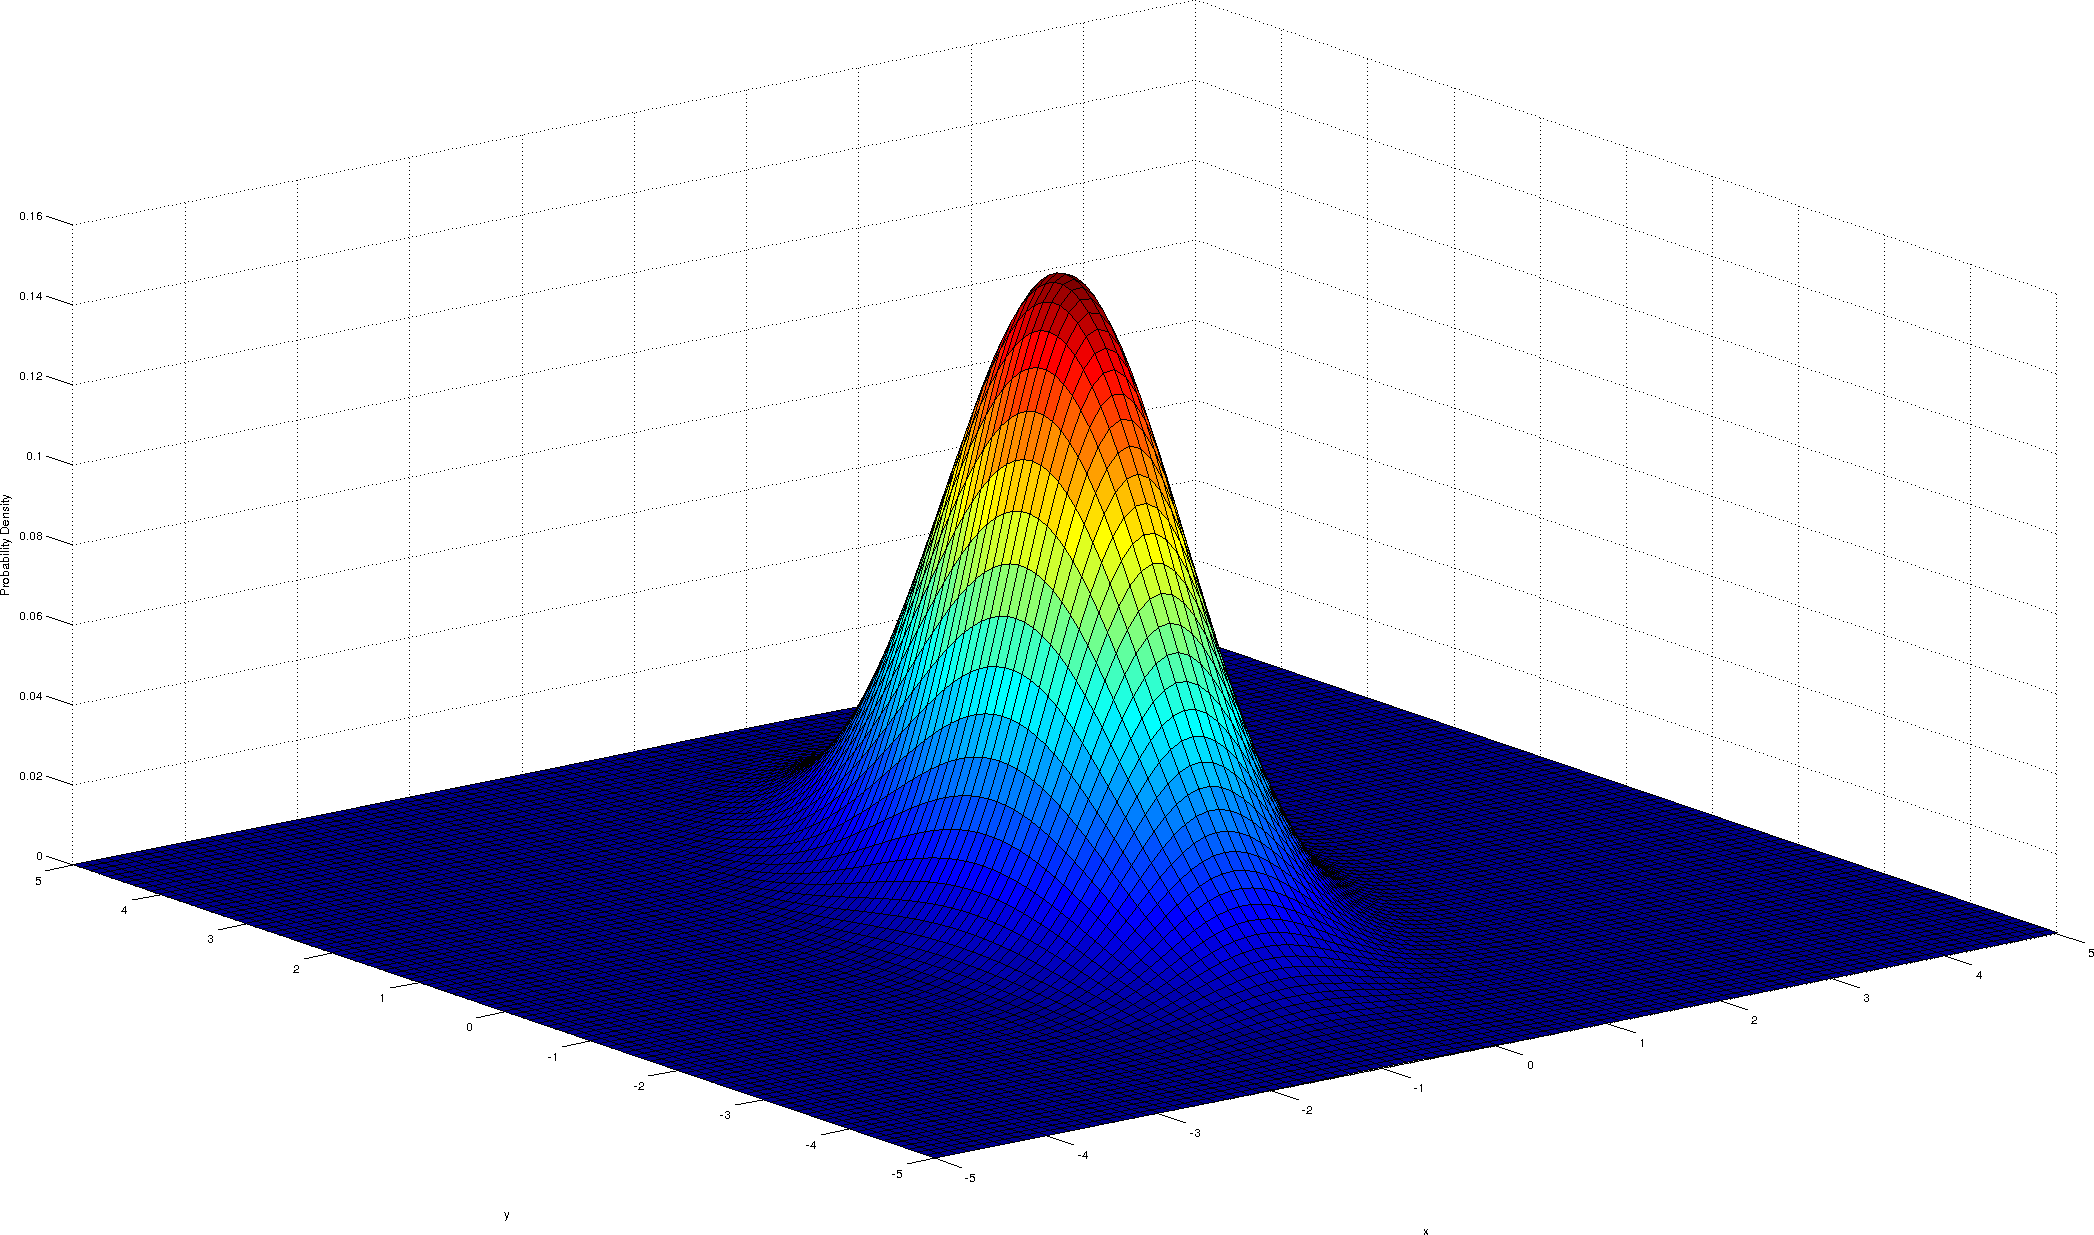
\includegraphics[width=\textwidth]{mvn_appendix_iso.png}
	\caption{caption goes here}
	\label{fig:some_nice_label_for_this_image}
\end{figure}



\begin{figure}[hptb]
        \centering
        \begin{subfigure}[b]{0.3\textwidth}
                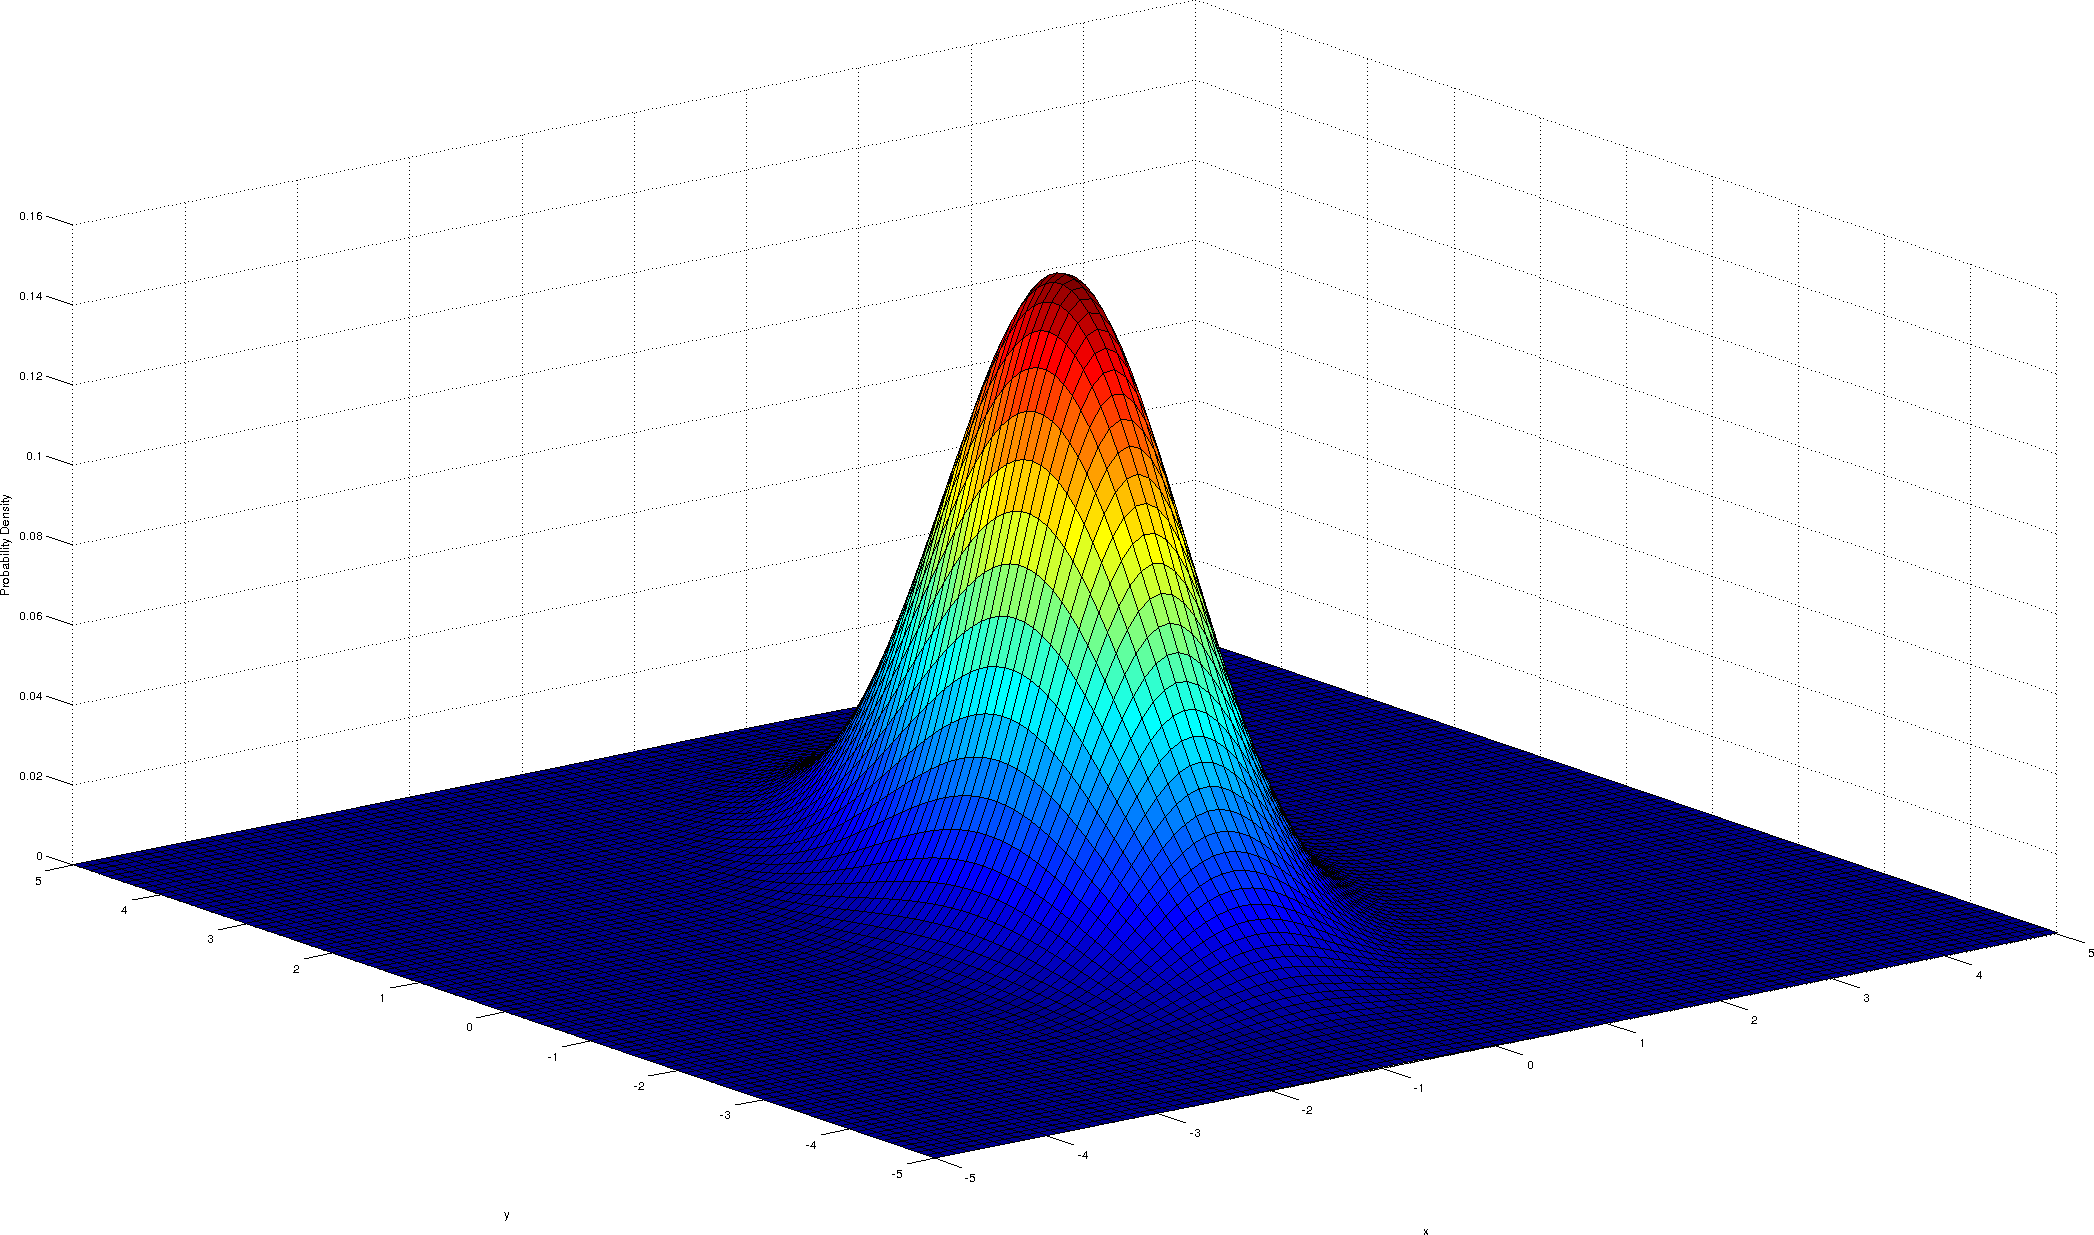
\includegraphics[width=\textwidth]{mvn_appendix_iso.png}
                \caption{caption}
                \label{fig:gull}
        \end{subfigure}%
        ~ %add desired spacing between images, e. g. ~, \quad, \qquad etc.
          %(or a blank line to force the subfigure onto a new line)
        \begin{subfigure}[b]{0.3\textwidth}
                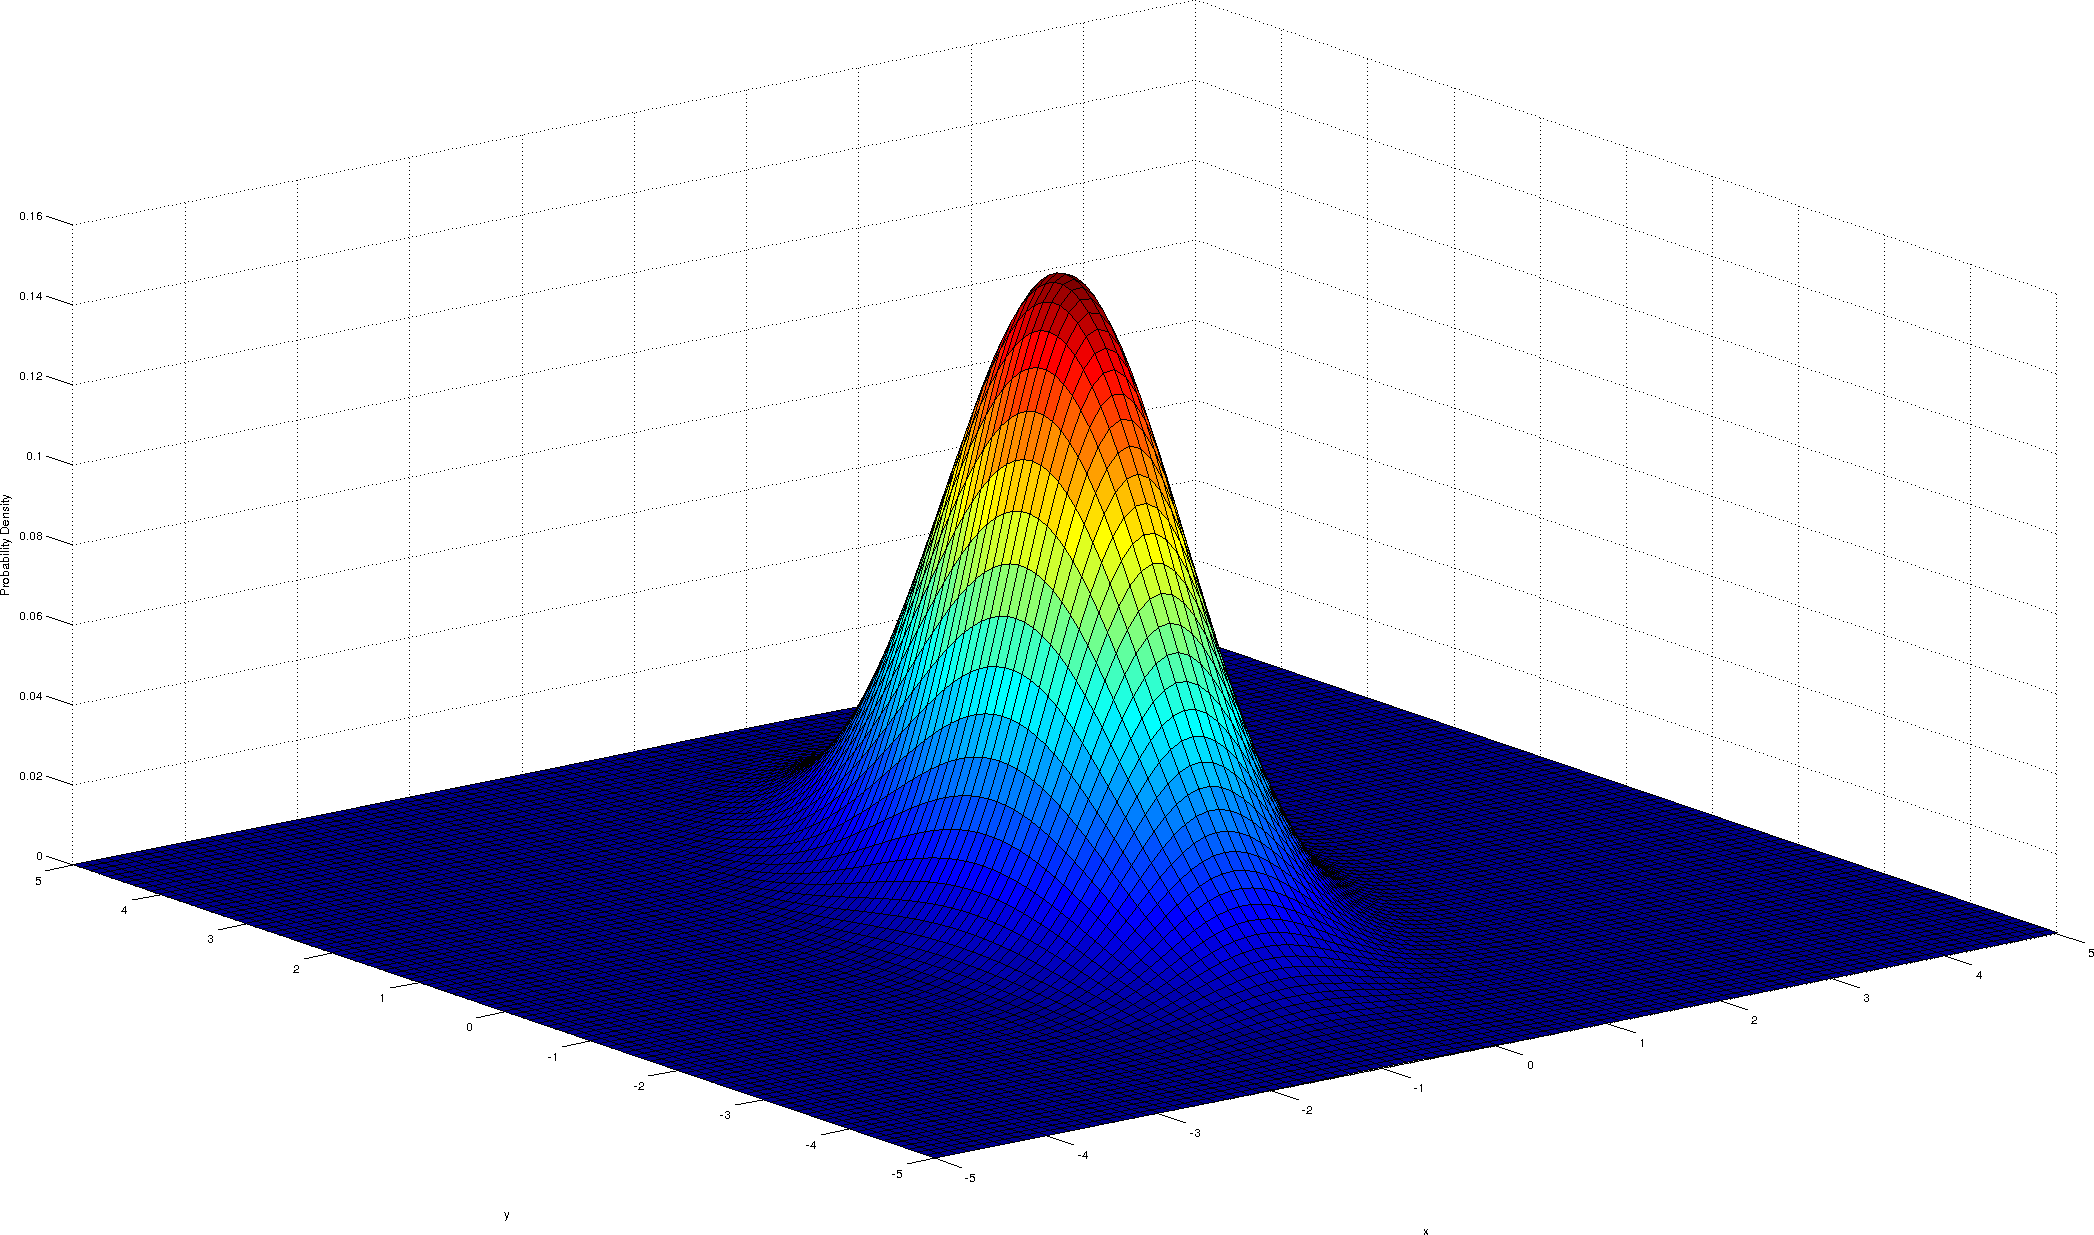
\includegraphics[width=\textwidth]{mvn_appendix_iso.png}
                \caption{caption}
                \label{fig:tiger}
        \end{subfigure}
        ~ %add desired spacing between images, e. g. ~, \quad, \qquad etc.
          %(or a blank line to force the subfigure onto a new line)
        \begin{subfigure}[b]{0.3\textwidth}
                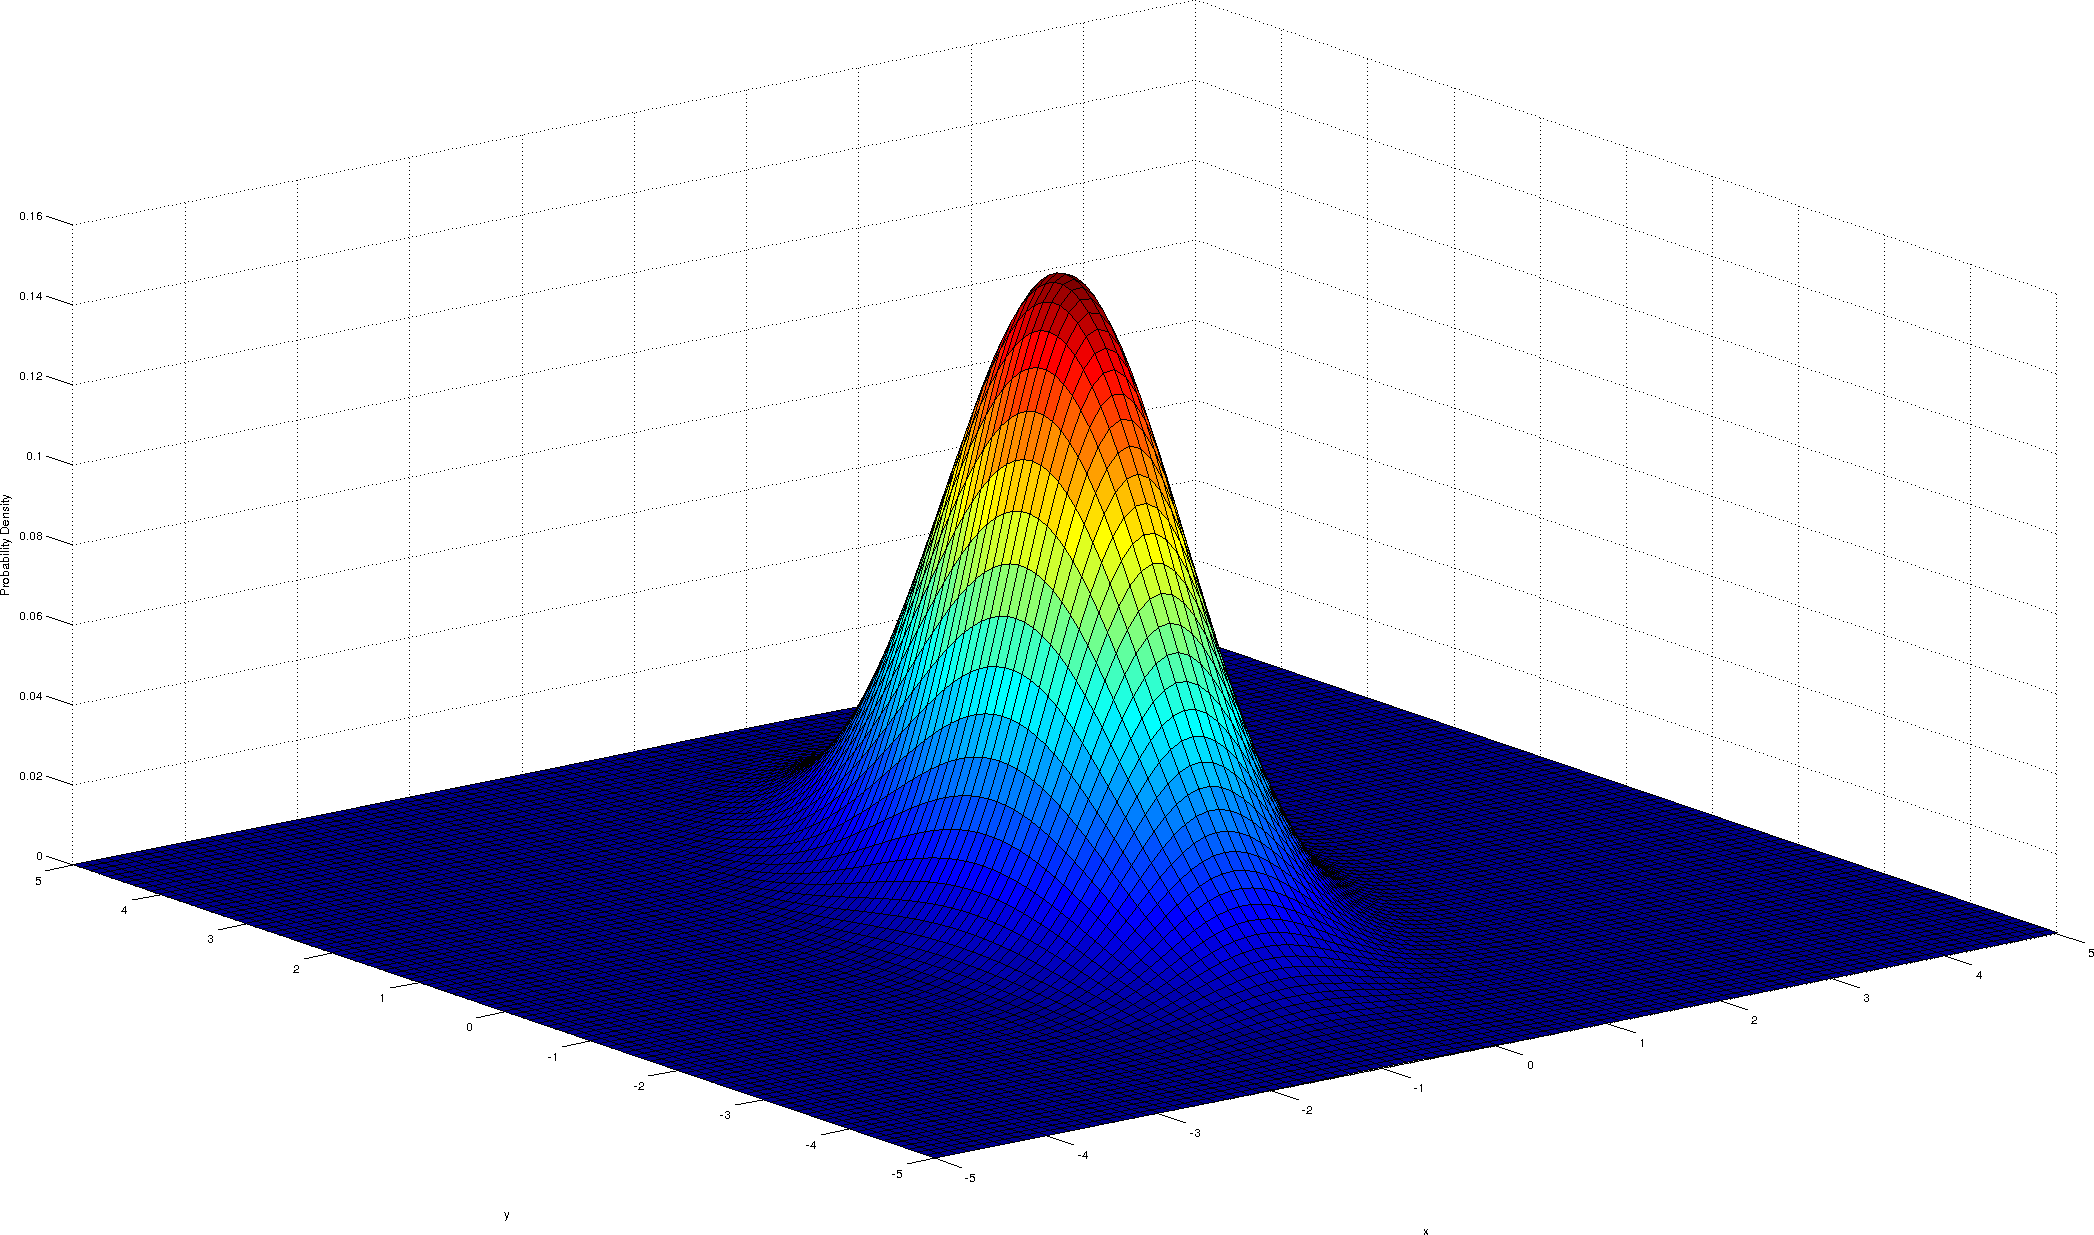
\includegraphics[width=\textwidth]{mvn_appendix_iso.png}
                \caption{caption}
                \label{fig:mouse}
        \end{subfigure}
        \caption{Pictures of something, horizontally}\label{fig:horizont}
\end{figure}



\begin{figure}[hptb]
	\centering
	\begin{subfigure}[t]{10cm}
		\centering
		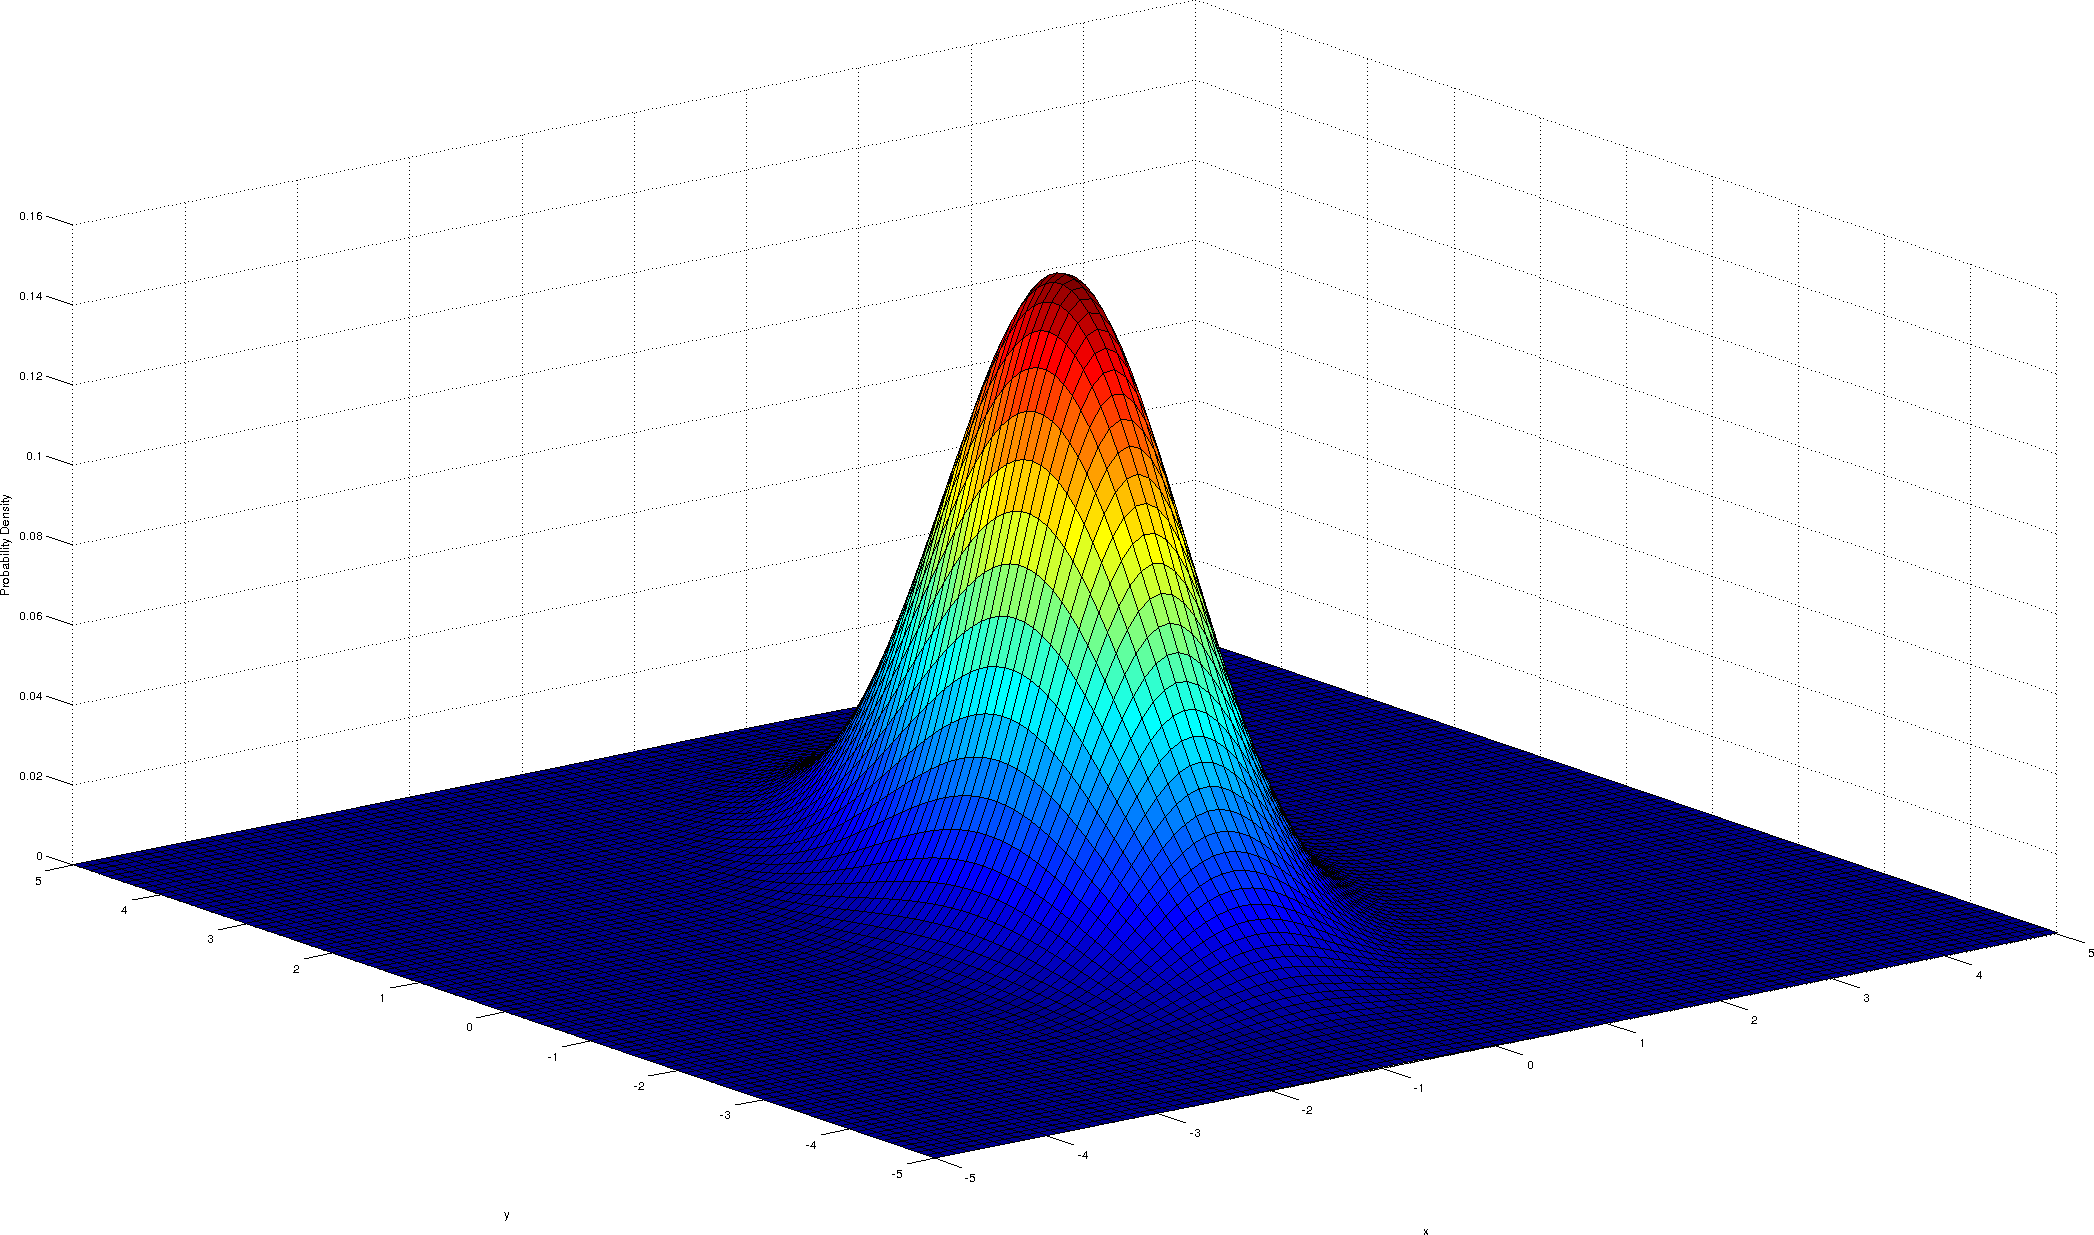
\includegraphics[width=10cm]{mvn_appendix_iso.png} 
		\caption{isometric perspective}
		\label{fig:app_mvn:iso}
	\end{subfigure}
	\begin{subfigure}[b]{\textwidth}
		\centering
		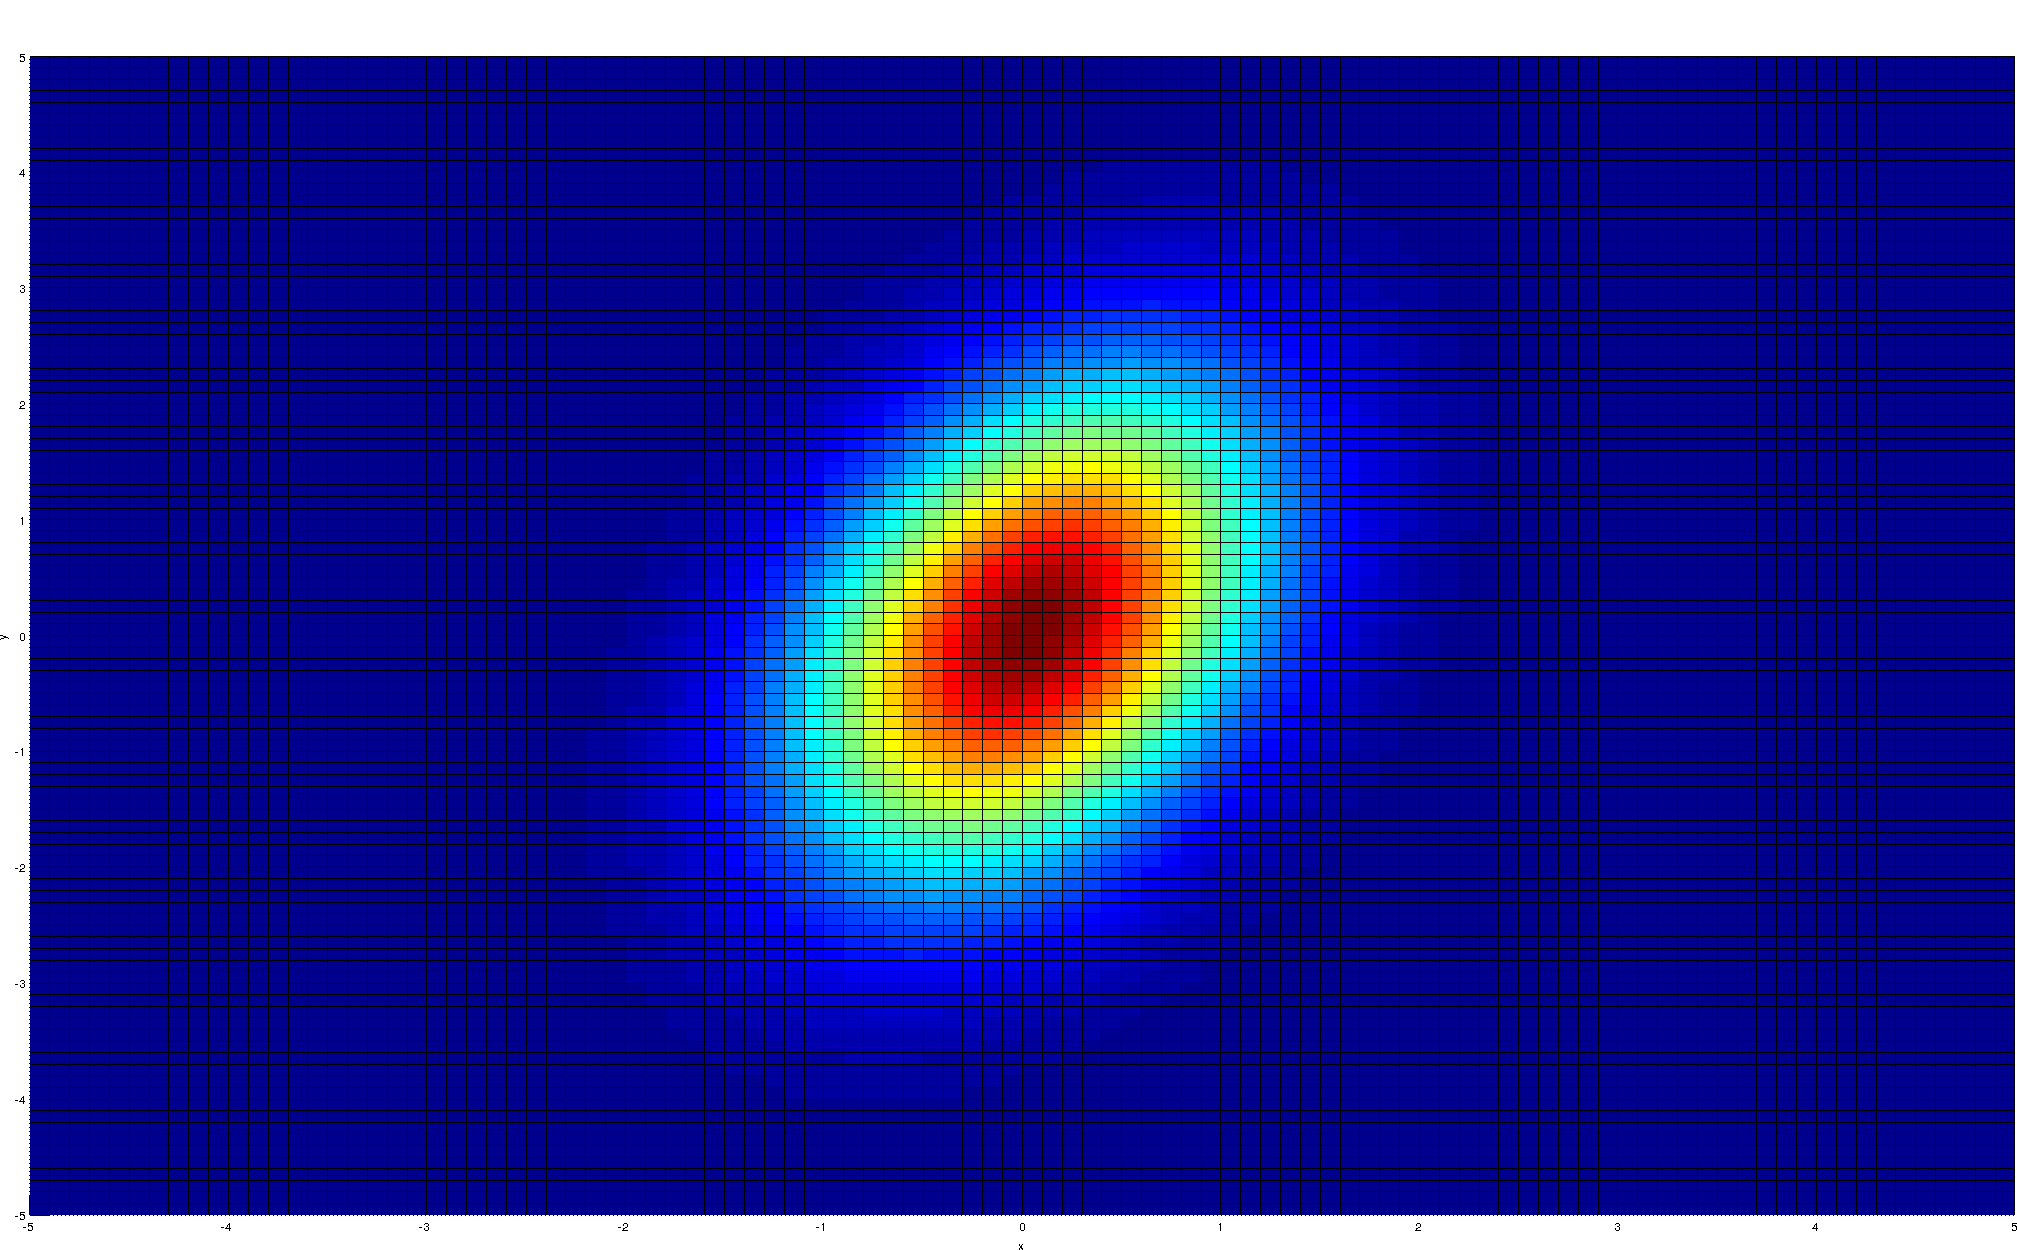
\includegraphics[width=10cm]{mvn_appendix_bird.png} 
		\caption{bird's eye view}
		\label{fig:app_mvn_bird}
	\end{subfigure}
	\caption[Multivariate Normal Distribution]{MVN with $\mu = \left[  
		\begin{array}{c} 
			0 \\ 
			0 
		\end{array} \right] $
		 and  $ \Sigma = \left[  
		\begin{array}{cc}
			0.6 & 0.4 \\ 
			0.4 & 2.0 \\
		\end{array} \right] $ }
	\label{fig:app_mvn}
\end{figure}







\newpage
\section{Math-Stuff}

Equations with explanations:
\begin{gather}
	p\left(x(k) \; \big| \; X^{k-1}, Z^{k-1}, U^k\right)
	\label{eq:bayes_1}
	\intertext{Where:}
	\begin{tabular}{>{$}r<{$}@{\ :\ }l}
		X^{k-1} := \{x(k-1), x(k-2), ..., x(0)\} & all previous states \\
		Z^{k-1} := \{z(k-1), z(k-2), ..., z(0)\} & all previous measurements \\
		U^k		:= \{u(k), u(k-1), ..., u(0)\} & all previous control inputs \\
	\end{tabular}\nonumber
\end{gather}

You can automatically refer to the beforehand stated equation~\ref{eq:bayes_1}. Pages with only math stuff sometimes looks strange. So make sure to add some nice text. 

\lipsum[0-1]


A list of equations aligned at the "=" symbol.
\begin{align}
	x(k+1|k) &= F(k) \cdot x(k|k) + G(k) \cdot u(k) 			\label{eq:kal_pred_x}	\\
	P(k+1|k) &= F(k) \cdot P(k|k) \cdot F(k)^T + Q(k) 			\label{eq:kal_pred_P}	\\
	\hat{z}(k+1|k) &= H(k+1) \cdot x(k+1|k) 					\label{eq:kal_pred_z}	\\
	S(k+1)   &= H(k+1) \cdot P(k+1|k) \cdot H(k+1)^T + R(k+1)	\label{eq:kal_pred_S}
\end{align}

References to Equation~\ref{eq:kal_pred_x} and  Equation~\ref{eq:kal_pred_z}

Write some matrices: $x = \begin{bmatrix}
x_{pos} \\
x_{vel} \\
y_{pos} \\
y_{vel}
\end{bmatrix}$ and $F = \begin{bmatrix}
1 & T & 0 & 0 \\
0 & 1 & 0 & 0 \\
0 & 0 & 1 & T \\
0 & 0 & 0 & 1
\end{bmatrix}$. 

\section{citing stuff}

You can cite stuff. For example an online resource \cite{adac_night}. Make sure to add a "laste visited" in JabRef. This has to appear in the bibliography. But you can also cite from a book, including the page number: \cite[p. 175]{mitchell1997}. And also inproceedings \cite{julier97} and articles \cite{Jin2003}. And technical manuals \cite{adma}.


\section{Tables}


\begin{table}[hbt]
	\begin{tabular}{p{4.0cm}C{3.6cm}C{4.0cm}}
		\toprule
		\textbf{Property}		&	\textbf{Stereo Camera}		&	\textbf{Multi-Mode Radar \newline (near / far)}	\\
		\midrule
		meas. principle	&	CMOS sensor			&	FMCW			\\
		cycle time		&	60ms				&	66ms			\\
		latency			&	42ms				&	198ms			\\
		\midrule
		frequency		&	16fps				&	76 - 77 Ghz		\\
		bandwidth		&	---					&	187 Mhz			\\
		\midrule
		opening angle	&	45°					&	60° / 18°			\\
		range			&	500m \newline (3D-vision: 50m)	&	~60m	/ 200m		\\
		\midrule
		angle accuracy ($3\sigma$)		&	---	&	~~$\pm$ 1° / $\pm$ 0.1°		\\
		distance accuracy ($3\sigma$)	&	---	&	$\pm$ 0.25m		\\
		velocity accuracy ($3\sigma$)	&	---	&	$\pm 0.278 \tfrac{m}{s}$ / $\pm 0.139 \tfrac{m}{s}$	\\
		\bottomrule
	\end{tabular}
	\caption{Overview of the properties of several sensors}
	\label{tab:sensor_properties}
\end{table}


\begin{table}[H]
	\centering
	\begin{tabular}{r|ccc|ccc}
	\toprule
       &  \multicolumn{3}{c|}{\textbf{full}}      & \multicolumn{3}{c}{\textbf{diag}}  \\
           &    RMSE &  PVol & NEES  & RMSE  & PVol & NEES        \\
    \midrule
    sensor-1    &    1.63   &  0.69 &  3.79   &    1.63 &   1.27 &     3.90     \\
    sensor-2    &    1.14   &  0.85 &  4.23   &    1.14 &   1.56 &     4.28     \\
    CMF         &    0.84   &  0.15 &  3.82   &    0.84 &   0.15 &     3.82     \\
  \midrule
    Naive       &    1.37   &  1.80 &  2.24   &    1.37 &   2.70 &     2.43     \\
    CI-trace    &    1.26   &  0.62 &  2.68   &    1.27 &   1.12 &     2.77     \\
    CI-det      &    1.37   &  0.61 &  3.31   &    1.34 &   1.11 &     3.16     \\
    Bar-Shalom-0.0      &    1.25   &  0.16 &  4.90   &    1.25 &   0.29 &     5.12     \\
    Bar-Shalom-0.4      &    1.21   &  0.25 &  4.04   &    1.22 &   0.46 &     4.09     \\
    Bar-Shalom-0.7      &    1.19   &  0.21 &  5.86   &    1.19 &   0.41 &     5.27     \\
    \midrule
    IMF         &    1.05   &  0.22 &  3.85   &    0.93 &   0.14 &     5.34     \\
    KF-T2T      &    1.80   & 12.17 & 7.15   &    1.64  &  11.76 &     5.32     \\
    IMF-sub     &    1.18   &  0.12 & 12.75   &    1.18 &   0.21 &    13.35     \\
	\bottomrule
	\end{tabular}
	\caption{some random numbers}
	\label{tab:res_prob1_vel_rmse}
\end{table}




\begin{table}[hbt]
\centering
\begin{small}
	\begin{tabular}{C{5.8cm}C{5.8cm}}
	\toprule
	\textbf{trainings set} & \textbf{validation set} \\
	\midrule
		$P_{C} = \begin{bmatrix}
			 0.307	&	 0.574	&	0	&	0	\\
			 0.574	&	 4.926	&	0	&	0	\\
			0	&	0	&	 0.052	&	 0.080	\\
			0	&	0	&	 0.080	&	 0.384	
		\end{bmatrix}$
		\newline
		$P_{R} = \begin{bmatrix}
			 0.066	&	 0.168	&	0	&	0	\\
			 0.168	&	 3.025	&	0	&	0	\\
			0	&	0	&	 0.360	&	 0.298	\\
			0	&	0	&	 0.298	&	 0.725	
		\end{bmatrix}$
		&
		$P_{C} = \begin{bmatrix}
			 0.301	&	 0.536	&	0	&	0	\\
			 0.536	&	 4.886	&	0	&	0	\\
			0	&	0	&	 0.054	&	 0.087	\\
			0	&	0	&	 0.087	&	 0.403	
		\end{bmatrix}$
		\newline
		$P_{R} = \begin{bmatrix}
			 0.071	&	 0.182	&	0	&	0	\\
			 0.182	&	 3.151	&	0	&	0	\\
			0	&	0	&	 0.356	&	 0.298	\\
			0	&	0	&	 0.298	&	 0.699	
		\end{bmatrix}$
\\
	\bottomrule
	\end{tabular}
\caption{covariances}
\label{tab:sol_stistical_emp_P_sim}
\end{small}
\end{table}




\section{Pseudo Algorithm}

For computer scientists: Write some pseudo code:

\begin{algorithm} 
	\begin{algorithmic}
		\Require $F$, $R$, $H$, $dt$ of the sensor
		\While {optimizing}
			\State select $q$
			\State calculate $P$ using alpha-beta equation
			\State calculate NEES
			\If {current NEES better than best NEES}
				\State $P_{ab} \gets P$
				\State best NEES $\gets$ current NEES
			\EndIf
		\EndWhile
		\State \Return {$P_{ab}$}
	\end{algorithmic}
	\caption{Pseudocode of the optimization process for $P_{ab}$}
	\label{algo:opti}
\end{algorithm} 

And explain it afterwards. 

\lipsum[1-2]



\section{Rotated Tables}
\vfill
\begin{center}
   \hvFloat[%
    nonFloat=true,%
    capPos=r,%
    capAngle=90,%
    capWidth=h,	% of \columnwidth
    capVPos=c,%
    objectAngle=90,%
]{table}{%
	% less padding around math environments
	\setlength{\abovedisplayskip}{50pt}	%
	\setlength{\belowdisplayskip}{50pt}	%
    \begin{tabular}{lL{2.5cm}L{10.5cm}c}	%
	\toprule
	 		& \textbf{needed data} & \textbf{equations} & \textbf{optimal}   \\ 
	\midrule
	CI 	
		&
		$ P_i$, $P_j $			\newline 
		$ \omega \in (0, 1) $
		&
		$ P^{-1} = \omega P_i^{-1} + (1 - \omega)P_j^{-1} $	\newline \vspace{5pt}
		$ \hat{x} = P \cdot [ \; \omega P_i^{-1}\hat{x}_i + (1 - \omega) P_j^{-1}\hat{x}_j \; ]$
		&	no		\\ 
	\midrule 
	BarS. 1				
		&	
		$P_i$ , $P_j$	\newline
		&	
		$ \hat{x} = P_j(P_i+P_j)^{-1}\hat{x}_i + P_i(P_i + P_j)^{-1}\hat{x}_j  $	\newline \vspace{5pt}
		$ P = P_1(P_i + P_j)^{-1}P_j $	
		&	no		\\ 
	\midrule 
	BarS. 2	
		&	
		$P_i$, $P_j$, $P_{ij}$, \newline
		$P_{ji}$, $K_i$, $K_j$, \newline
		$H_i$, $H_j$, 			
		$F$, $Q$
		&	
		$ \hat{x} = \hat{x}_i + [P_i - P_{ij}][P_i + P_j - P_{ij} - P_{ji}]^{-1}[\hat{x}_j - \hat{x}_i] $	 \newline \vspace{5pt}
		$ P = P_i - [P_i - P_{ij}][P_i + P_j - P_{ij} - P_{ji}]^{-1}[P_i - P_{ji}]$	\newline \vspace{5pt}
		$ P_{ij} \approx 0.4 \cdot \sqrt{P_i \circ P_j} $
		&	yes		\\ 
	\midrule
	IMF 			
		&
			$\hat{x}_i(k|k-1)$	\newline
			$\hat{x}_i(k|k)$		\newline
			$P_i(k|k-1)$			\newline
			$P_i(k|k)$			\newline
			$ \hat{x}(k|k-1) $	\newline
			$ P(k|k-1)$			\newline
			$F$, $Q$
		&	
		\newline 
		$ P(k|k)^{-1} = \sum_{i=1}^2 \left[ P_i(k|k)^{-1}  - P_i(k|k-1)^{-1} \right]  + P(k|k-1)^{-1} $	\newline \vspace{5pt}
		$ \hat{x}(k|k) = P(k|k) \cdot \{ \; P(k|k-1)^{-1} \cdot \hat{x}(k|k-1)  $	\newline \vspace{5pt}
		$	 \qquad	\qquad		 + \sum_{i=1}^2 \left[ P_i(k|k)^{-1} \hat{x}_i(k|k) - P_i(k|k-1)^{-1} \hat{x}_i(k|k-1) \right] \; \}	$
		&	yes		\\
	\bottomrule
    \end{tabular}
}[hpbt]{Summary of the used track-to-track fusion algorithms}{tab:t2t_summarytable}
\end{center}
\vfill\clearpage


\chapter{Final Discussion}
\label{c:final_discussion}

This chapter summarises the experimental results in an overall context and suggestions for further research are given.

\section{Consolidation}
\label{s:consolidation}

Summary of the Thesis. What has been studied, what has been found. Be critical with you own results here once again. At the very end, sum your whole thesis up in 2 sentences


In this Master Thesis ... has been studied. As a first experiment ... . As a result ... . However, ... . Further research is needed ... .

Furthermore, ... . 

To sum it up, ... .


\section{Future Research}
\label{s:futureresearch}

Give suggestions about future research to overcome the limitations of this work. What could and should be done.

















\chapter{Appendix}
\label{c:appendix}

supplementary material goes here.

\section{Derivations}
\label{s:appendic_derivations}

add some derivations here.


\newpage
\subsection{Example Matlab Code}
\label{ss:app_kalman_matlab}

Add a sourcefile directly into \LaTeX

\lstinputlisting[label={src:SimpleKalmanExample}, caption={Simple example of a Kalman Filter in Matlab}]{simple_kalman_example.m}













% acknowledgement is done directly is this file. see below
% bibliography is done directly is this file. see below



%%% Acknowledgement
\cleardoublepage
\chapter*{Acknowledgement}
\label{c:acknowledgement}

First of all, I would like to express my gratitude to ... for the aspiring guidance, useful comments and invaluably support throughout the whole process of this Master Thesis. Furthermore, I would like to thanks ..., ... and the other members of the research team for helpful discussions and constructive criticism. In addition, I would like to thank my University supervisor ... for all the helpful remarks, advises and discussions.

Also, I would like to thank my parents and ... who have supported me throughout the entire process by keeping me harmonious and motivated. 

Last but not least, I like to thank ... for funding my research and providing me with the facilities being required.



%%% list of all figures in this thesis
\listoffigures



%%% bibliography // references
\cleardoublepage
\bibliographystyle{abbrvnat}
\bibliography{papers}



%%% closing - conformation on non-cheating
\cleardoublepage
\chapter*{Proclamation}
Hereby I confirm that I wrote this thesis independently and that I have not made use of any other resources or means than those indicated.
\bigskip\bigskip\bigskip\bigskip\bigskip\bigskip\bigskip\bigskip
\begin{flushright}
	Forname Surname, Place, \today
\end{flushright}



\end{document}




































